\section{Experiments}
\label{sec:experiments}

The objective of this experiment section is threefold:
\begin{itemize}
\item To show the evolution of the average neighborhood size of members of an
  editing session. Using \SPRAY, we expect a logarithmic growth compared to the
  global size of the network.
\item To confirm the complexity analysis of \LSEQ. Concerning the size of
  identifiers, the common monotonic editing behavior should lead to a
  polylogarithmic growth compared to the document size. Concerning the time
  complexities, they should be logarithmic except for the look-up. This latter
  should be linear after monotonic editing behavior.
\item To show that both the identifier size and neighborhood size impact the
  traffic. Since the former grows polylogarithmically, and the latter grows
  logarithmically, we expect the traffic to scale in terms of number users and
  number of operations.
\end{itemize}

We conducted the experiments using a Javascript implementation directly usable
within modern web browsers\footnote{https://github.com/Chat-Wane/CRATE}. The
experiments ran on the \emph{Grid'5000} testbed involving uptil 601 instances of
the editor distributed among 101 machines.

\ \\ 

\begin{figure}
  \centering
  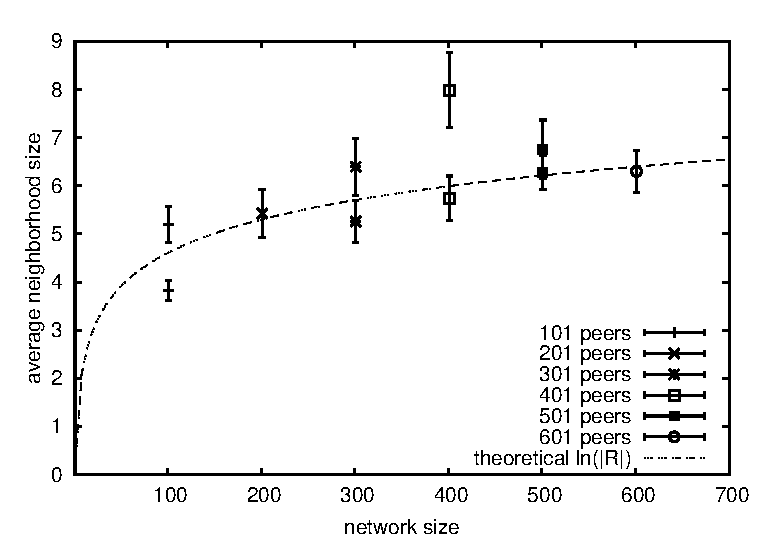
\includegraphics[width=0.475\textwidth]{./img/partialview.eps}
  \caption{\label{fig:partialview} Average neighborhood size of each peer over
  the global network size.}
\end{figure}

\begin{asparadesc}
\item [Objective:] To show the evolution of the average neighborhood size of
  members of an editing session. The \SPRAY protocol aims to provide a
  logarithmically scaling neighborhood compared to the global network
  size. Furthermore, the protocol builds a dynamic network where the load is
  balanced among members.
\item [Description:] During a run, peers dynamically modify their
  neighborhood. Each peer periodically reports its neighborhood size. Then, we
  average all these values and measure the variance. The average value defines
  how connected is a member to the network, impacting (among other) on the
  information dissemination efficiency. The variance defines how spread are the
  values; a small value means a good load balancing among members. Runs comprise
  from 101 members to 601 members with 100 members increments, i.e., 6 different
  runs.  The first member creates the editing session which is progressively
  joined by the other writers (1 joiner per 5 seconds). Each member starts
  sharing the document as soon as its joining. Hence, outsiders can join the
  network through one of them chosen at random.
\item [Results:] Figure~\ref{fig:partialview} shows the results of this
  experiment. The figure displays the network size on the x-axis and the average
  neighborhood size on the y-axis. It shows the average value of each experiment
  along with the theoretical expectation: a natural logarithm on the global
  network size. Each average value also carries the variance measurement. As
  expected, we observe that the average neighborhood size grows logarithmically
  compared to the size of the network despite being scattered around the
  theoretical curve. Figure~\ref{fig:partialview} also shows that the variance
  is small around the average values. Thus, members have an even neighborhood
  size. In other terms, the load is well-balanced among members when they need
  to disseminate information to the whole network. At the opposite of
  centralized solutions, it builds a topology where no member is more important
  than another in term of connectivity. As such, the network is more resilient
  to random crashes or unexpected departures.
\item [Reasons:] When an outsider wants to join the editing session, it picks a
  random sharer as first contact. \SPRAY assumes that the neighborhood size of
  this particular member is already logarithmic compared to the network
  size. Therefore, it uses this assumption to create additional connections that
  increase logarithmically in number. Yet, the averages neighborhood size does
  not follow exactly the theoretical expectation curve. Indeed, the number of
  neighbors of each member strongly depends of the first contact. However, the
  specific average value is not necessarily reached, especially considering
  that, while the theoretical expectation is a floating number, the neighborhood
  size belongs to the integers. This fact also impacts the variance. Indeed, the
  \SPRAY protocol exchanges the neighborhood of member over time. During the
  exchanges, it aims to balance the neighborhood size of each peer. Yet, the
  average value may not be an integer value. Therefore, the neighborhood size of
  the members constantly fluctuates around the average value.
\end{asparadesc}

\ \\

\begin{figure}
  \centering
  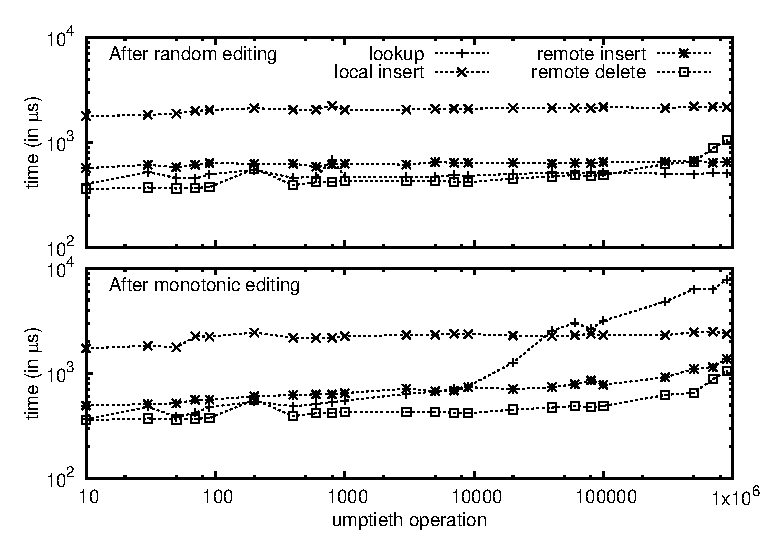
\includegraphics[width=0.475\textwidth]{./img/bench.eps}
  \caption{\label{fig:bench} Time performance of operations.}
\end{figure}

\begin{asparadesc}
\item [Objective:] To confirm the time complexity of the operations of
  \LSEQ. The time complexity part of Table~\ref{table:lseqtime}
  summarizes our expectations.
\item [Description:] This experiment involves one user who performs operations
  on its local copy of the document. The benchmark ran on a MacBook Pro with 2.5
  GHz Intel Core i5, with Node.js 4.1.1 on Darwin 64-bit. To each operation, we
  create a document containing $I-1$ characters and measure the time taken by
  the $I^{th}$ operation. The operation set includes the look-up, the local part
  of an insertion, the remote part of an insertion, and the remote part of a
  deletion. We perform the measurements multiple times on two kinds of
  documents. Firstly, a document generated by random editing (i.e. the
  underlying \LSEQ tree is balanced). Secondly, a document generated by
  monotonic editing (i.e. one branch per level of the \LSEQ tree is filled).  We
  focus on tendencies rather than absolute values. Javascript does a lot of
  on-the-fly optimization which we limit in order to show the real time
  contribution of each operation.
\item [Results:] Figure~\ref{fig:bench} shows the result of this experiment. The
  x-axis denotes the number of insert operations performed before the measured
  operation. The y-axis denotes the average time taken by this operation. The
  top part of the figure focuses on a structure filled with insertions following
  a random editing behavior while the bottom part of the figure focuses on a
  structure filled with insertions following a monotonic editing behavior. We
  observer that the measured values barely grow after random editing, regardless
  of the operation. On the other hand, while the local insertion after monotonic
  editing remains stable, we observe a linear growth with the look-up execution
  time, and a slower growth for both the remote insertions and the remote
  deletions.
\item [Reasons:] After the insertions at random positions, the underlying tree
  of \LSEQ is balanced. Therefore, the range of influence of each operation is
  limited to a small subset of the elements composing the document. For
  instance, the look-up operation does not need to explore each element of the
  tree. Instead, it quickly discards a lot of irrelevant branches at each level
  of the tree because the index does not fall into their range. However, this
  remark does not hold when the insertions followed a monotonic editing
  behavior. Indeed, in this case, most elements are located in the one and
  deepest level of the tree. Thus, the look-up likely crawls to this level and
  then inspects each elements to count their children and actualize its current
  index. The remote operations measurements follow the same reasoning: they must
  perform a binary search at each depth of the tree; since the random editing
  structure is balanced, the average depth of the search is smaller compared to
  the structure resulting from monotonic editing behavior. Hence, a lower time
  complexity.
\end{asparadesc}

\ \\

\begin{figure}
  \centering
  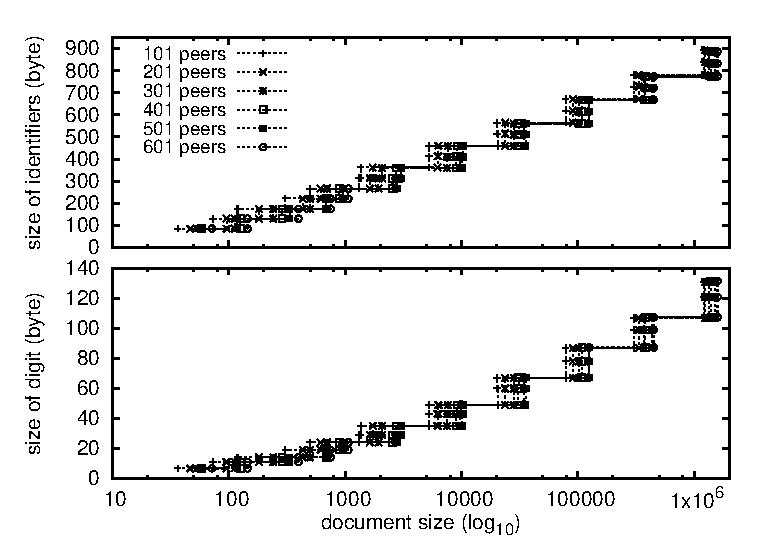
\includegraphics[width=0.475\textwidth]{./img/identifiers.eps}
  \caption{\label{fig:identifiers} Average size of identifiers.}
\end{figure}

\begin{asparadesc}
\item [Objective:] To confirm the space complexity of the identifiers generated
  by \LSEQ. On the common monotonic editing behavior, we expect a
  polylogarithmic growth compared to the document size.
\item [Description:] The executions follow the previous experiment about the
  neighborhood size. Thus, the experimentation comprises 6 runs with networks
  including 101, 201, 301, 401, 501, 601 members. The editing session members
  are repeatedly inserting new characters at the end of the document. The rate
  of these operation is 100 operations per second distributed among
  members. Thus, the experiment involving 101 members forces each member to
  perform 1 insertion per second, while the experiment involving 601 members
  forces each member to perform 1 insertion every 6 seconds. During the runs,
  each author reports the byte-size of newly generated identifiers along with
  the byte-size of its path in the exponential tree. \TODO{site, counter,
    starting values of the exponential tree}.
\item [Results:] Figure~\ref{fig:identifiers} shows the result of this
  experimentation. The x-axis denotes the document size (which is equivalent to
  the number of insert operations since the members do not perform removals) on
  a decimal logarithmic scale. Thus, the document grows from empty to above a
  million characters. The y-axis of the top part of the figure denotes the
  byte-size of the identifiers while the bottom part of the figure denotes the
  byte-size of the path only. First, we observe that all plots are very close
  from each other. Hence, the size of identifiers does not depend of the number
  of participants. Second, we observe that the identifiers grows
  polylogarithmically compared to the size of the document. Indeed, the bottom
  part of Figure~\ref{fig:identifiers} shows that the increment step of the
  generated paths is slowly increasing during the experiment. It empirically
  exposes a small surlinear behavior when the x-axis is on a logarithmic
  scale. Hence the polylogarithmic curve. Finally, we can observe that \LSEQ
  generates paths the size of which is small comparatively to the whole
  identifier that includes site identifiers and counters to guarantee
  uniqueness.
\item [Reasons:] The curves of the byte-size are close because the identifiers
  of \LSEQ do not depend of whom created it nor the number of authors involved
  in the document editing. They only depend of the position of insertions which
  globally corresponds to the editing behavior. In this case, the highlighted
  editing behavior is a monotonic left-to-right editing, i.e., repeated
  insertions at the end of the document. This kind of behavior tends to
  unbalance the tree by filling only one branch per level of the
  tree. Fortunately, since the tree exponentially grows (each element has twice
  as much children as its parent), the path growth slowly decreases over
  insertions. Nevertheless, it costs one additional bit to encode each
  concatenation of the path, hence the path growth on the bottom part of the
  figure. The identifiers are much heavier than the path they carry because they
  also includes a list of pairs to guarantee the uniqueness of identifiers and a
  global total order. Each member generates its own globally unique identifier
  (with high probability) without relying on any remote service. As such, they
  require large identifiers that does not collide with remote members.
\end{asparadesc}

\ \\

\begin{figure}
  \centering
  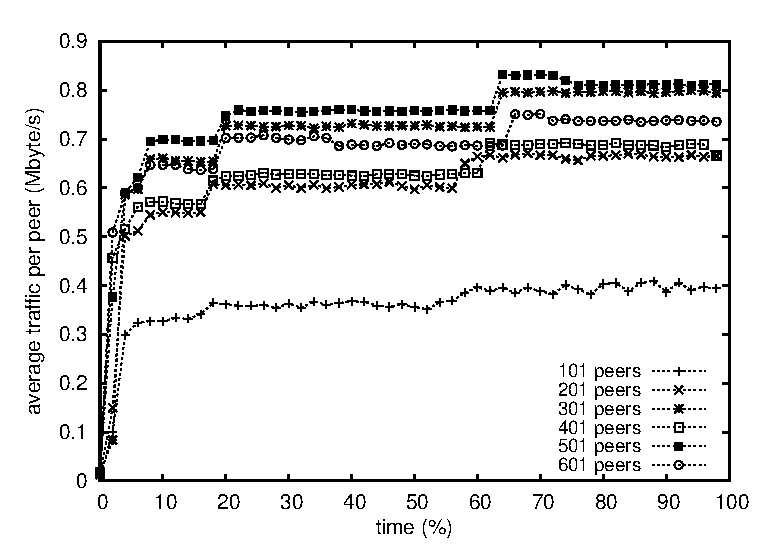
\includegraphics[width=0.475\textwidth]{./img/traffic.eps}
  \caption{\label{fig:traffic} Average traffic per second at each peer
    during the experiments.}
\end{figure}

\begin{asparadesc}
\item [Objective:] To show that both the identifier size and neighborhood size
  impact the traffic. Since the former grows polylogarithmically, and the latter
  grows logarithmically, we expect the traffic to scale in terms of number of
  users and number of operations.
\item [Description:] As for prior experiments, this experimentation concerns
  networks from 101 members to 601 members, each coauthoring a document of over
  a million of characters by repeatedly inserting new characters at the end of
  the document. Figure~\ref{fig:partialview} displays the average neighborhood
  size of members of each run. Figure~\ref{fig:identifiers} displays the
  identifiers size of each run. This experiment measure average traffic of
  members in Megabyte per second. For the recall, 100 operations are performed
  per second uniformly distributed among participants.
\item [Results:] Figure~\ref{fig:traffic} shows the result of this experiment.
  The x-axis denotes the experiment progression. The y-axis shows the average
  outgoing traffic generated by members (in Megabyte per second). As expected,
  we observe three results:
  \begin{inparaenum}[(i)]
  \item It confirms the results of both prior experiments about the neighborhood
    size (i.e., a logarithmically growing/shrinking neighborhood size compared
    to the network size), and the size of identifiers (i.e. a
    polylogarithmic growth compared to the size of the document).
  \item Being adaptive, the \SPRAY membership protocol grants the ability to
    disseminate information scaling with the network dimension.
  \item The growth of identifiers constitutes an important part of the traffic
    as well.
  \end{inparaenum}
  Hence, \CRATE scales in terms of number of users and number of operations.
\item [Reasons:] When an outsider joins the network, it injects a number of
  connections roughly logarithmic compared to the current network size. When it
  generates an operation, it sends its result to its neighborhood. Since this
  result (i.e. the identifier) grows polylogarithmically compared to the
  document size, and since the neighborhood grows logarithmically compared to
  the network size, it multiplies the polylogarithm with the logarithm. When a
  member receives such operation, and it receives it for the first time, it
  sends it to its neighborhood. Therefore, for each operation performed by any
  member, the rest of the members will send the result of the operation to all
  their respective neighborhood once. As such, the network load is balanced
  among users. Furthermore, it scales in number of editing session members and
  document size.
\end{asparadesc}

%%% Local Variables:
%%% mode: latex
%%% TeX-master: "../paper"
%%% End:
